\chapter{Benchmark Nominal e Resposta a Perturbações}
\label{cap:benchmark}

Neste capítulo, é apresentado o protocolo de simulação utilizado para a avaliação do desempenho dos controladores PID aplicados ao Reator Contínuo de Tanque Agitado (CSTR). Subsequentemente, analisam-se os resultados sob diferentes métodos de sintonia.

\section{Protocolo de Simulação}
\label{sec:protocolo_simulacao}

A integração das equações diferenciais ordinárias (EDOs) do modelo do CSTR foi realizada através do solver \texttt{solve\_ivp} da biblioteca SciPy, utilizando o método numérico de Dormand-Prince de ordem 4(5) (RK45). A tolerância relativa foi definida como \num{1e-10} e a tolerância absoluta como \num{1e-12}, garantindo precisão adequada para sistemas com dinâmicas acentuadamente não lineares e rápida evolução temporal. O tempo de amostragem do sistema de controle digital foi estabelecido em $\Delta t = \SI{0.02}{\minute}$ (ou seja, \num{50} amostras por minuto), adequado às constantes de tempo do processo térmico.

O cenário de teste padronizado consiste na aplicação de uma perturbação tipo degrau na referência (setpoint) de temperatura, denotada por $\Delta T_{sp} = \SI{+5}{\kelvin}$, partindo do estado estacionário em $T = \SI{396.65}{\kelvin}$ para \SI{401.65}{\kelvin} no instante $t = \SI{0}{\minute}$. A fim de avaliar a capacidade de rejeição a distúrbios, impõe-se uma perturbação degrau na temperatura de alimentação $\Delta T_{f} = \SI{+10}{\kelvin}$ no instante $t = \SI{10}{\minute}$.

Para quantificar objetivamente o desempenho das estratégias de controle em malha fechada, os seguintes índices e métricas foram computados:
\begin{itemize}
    \item Integral do Erro Absoluto (IAE) e Integral do Erro Absoluto Ponderado pelo Tempo (ITAE);
    \item Integral do Erro Quadrático (ISE);
    \item Sobressinal máximo ($M_p$), expresso em porcentagem;
    \item Tempo de acomodação ($t_s$) para uma banda de \SI{2}{\percent};
    \item Variação Total da ação de controle (TV), definida como $\text{TV} = \sum |u(k) - u(k-1)|$, utilizada como métrica heurística do desgaste do atuador (válvula).
\end{itemize}

O Código~\ref{lst:compute_metrics} apresenta a implementação computacional desenvolvida para a extração rigorosa de tais métricas a partir das trajetórias simuladas.

\begin{lstlisting}[language=Python, caption={Cálculo das métricas de desempenho em malha fechada.}, label={lst:compute_metrics}]
def compute_metrics(
    time: NDArray[np.float64],
    error: NDArray[np.float64],
    output: NDArray[np.float64],
    setpoint: NDArray[np.float64],
    tolerance_pct: float = 2.0,
) -> PerformanceMetrics:
    # Compute the average sampling time
    dt = float(np.mean(np.diff(time)))
    step_size = float(setpoint[-1] - setpoint[0])
    
    # Calculate integral performance indices
    ise = float(np.trapz(error**2, time))
    iae = float(np.trapz(np.abs(error), time))
    itae = float(np.trapz(time * np.abs(error), time))
    
    # Calculate peak metrics
    if step_size != 0:
        peak = float(np.max(output) if step_size > 0 else np.min(output))
        overshoot_pct = max(0.0, (peak - setpoint[-1]) / abs(step_size) * 100)
    else:
        overshoot_pct = 0.0
        
    # Placeholder for settling time, rise time, and steady-state error extraction
    # ...
    
    return PerformanceMetrics(ise=ise, iae=iae, itae=itae, overshoot_pct=overshoot_pct)
\end{lstlisting}
\vspace{2pt}\par\noindent{\footnotesize\textbf{Fonte:} Elaborada pelos autores (2026).}

\section{Desempenho sob Sintonia Ziegler-Nichols}
\label{sec:desempenho_zn}

A avaliação dos parâmetros derivados do método clássico de resposta em malha aberta de Ziegler-Nichols \cite{ZieglerNichols1942} culminou em falha catastrófica de estabilização. Observou-se um sobressinal $M_p > \SI{800}{\percent}$, acompanhado por um $\text{IAE} > 100$ e episódios estendidos de saturação contínua e persistente na vazão de líquido refrigerante ($u_{\max} = \SI{300}{\liter\per\minute}$).

Tais anomalias refletiram-se em excursões de temperatura inaceitáveis, ultrapassando \SI{+56.5}{\kelvin} em relação à nova referência, conduzindo o reator em direção ao limiar do colapso térmico (\textit{thermal runaway}). O mecanismo elementar dessa falha pode ser atribuído à realimentação positiva gerada entre os ganhos excessivamente agressivos propostos pelo critério heurístico e a forte dependência exponencial cinética intrínseca à equação de Arrhenius \cite{Fogler2016}.

Neste cenário de falha aguda, o controlador passou a demandar substancialmente mais refrigeração do que o máximo fisicamente viável. A aplicação do método de \textit{anti-windup} limitou momentaneamente os desvios, porém a extensão do dano térmico já se encontrava irreversivelmente configurada pela própria natureza reativa do sistema \cite{Bequette2003}.

\section{Desempenho sob Sintonia Cohen-Coon}
\label{sec:desempenho_cc}

Conforme reportado na Seção \ref{sec:desempenho_zn}, os efeitos observados com a aplicação do critério de sintonia de Cohen e Coon \cite{CohenCoon1953} resultaram em um desempenho notavelmente inferior em comparação direta com os resultados obtidos através da metodologia Ziegler-Nichols. O ganho proporcional $K_p$ fornecido pelo método é significativamente mais agressivo, o que resultou em sobressinais de maior amplitude e períodos prolongados de operação sob o regime de saturação restrita do atuador térmico.

Os resultados evidenciam categoricamente a inadequação fundamental de ambas as metodologias clássicas de natureza estritamente linear no que concerne à estabilização operacional em circuito fechado de plantas reacionais caracterizadas por instabilidade intrínseca de malha aberta (polos instáveis) e pronunciada não-linearidade térmica de primeira ordem, um cenário ubíquo em engenharia das reações químicas \cite{Luyben2007}.

\section{Desempenho sob Sintonia SIMC (Skogestad)}
\label{sec:desempenho_simc}

A síntese do controlador baseada no modelo interno pelo método de redução analítica simples proposta por Skogestad (SIMC) \cite{Skogestad2003} apresentou uma \textit{performance} formidável. Um expressivo índice $\text{IAE} = 1.09$ foi registrado, simultaneamente à ocorrência de um modesto sobressinal $M_p = \SI{2.1}{\percent}$ e da observação de um sinal de controle consideravelmente suave, estritamente confinado ao intervalo exequível $u \in [40, 220]\,\SI{}{\liter\per\minute}$.

Destaca-se a exímia aptidão da malha de controle na anulação ativa e tempestiva dos efeitos nocivos resultantes da perturbação imposta em $T_f$, viabilizando a regressão à referência almejada em um intervalo correspondente a aproximadamente $\SI{3}{\minute}$. A Variação Total (TV) associada ao esforço manipulativo permaneceu confinada em limites razoáveis, implicando a preservação física das válvulas proporcionais ao longo do ciclo operacional \cite{Seborg2016}.

\section{Desempenho sob Sintonia ITAE Ótima}
\label{sec:desempenho_itae}

Com o intuito de mitigar as penalidades ao longo do tempo prolongado (via peso na variável integradora $t$), a busca do mínimo paramétrico estrito pelo índice ITAE revelou ser a configuração possuidora da otimalidade integral superior. Computou-se $\text{IAE} = 0.89$, tolerando um suave crescimento do sobressinal para $M_p = \SI{4.8}{\percent}$, além do índice sensibilidade correspondendo a $M_s = 1.24$, atestando adequadas margens de robustez.

Essa configuração exibe dinâmicas ligeiramente mais incisivas nas ações de restabelecimento na fronteira das transições que a sua contraparte SIMC. Notou-se elevação modesta da TV em face do esforço mais agressivo exigido sobre o manipulador; entretanto, a considerável redução do valor integral temporal global (IAE) frequentemente justifica esse pequeno acréscimo em detrimento térmico da planta em aplicações da vida real \cite{Shinskey1996,Astrom2006}.

\section{Tabela Comparativa de Métricas de Desempenho}
\label{sec:tabela_metricas}

A \autoref{tab:metricas_desempenho} congrega, de forma estruturada e sintetizada, os resultados provenientes do mapeamento das matrizes simuladas relativas às metodologias investigadas. Adicionalmente, a \cref{fig:benchmark_completo} ilustra com exatidão as trajetórias dinâmicas temporais da temperatura do reator $T(t)$ e da vazão de resfriamento $q_j(t)$ para os quatro controladores, evidenciando o contraste marcante entre a estabilização robusta assegurada por SIMC e ITAE contra a divergência com saturação crônica induzida por Ziegler-Nichols e Cohen-Coon.

% fig_benchmark.tex - Grafico comparativo de transientes
\begin{figure}[htbp]
\centering
\begin{subfigure}{\textwidth}
\centering
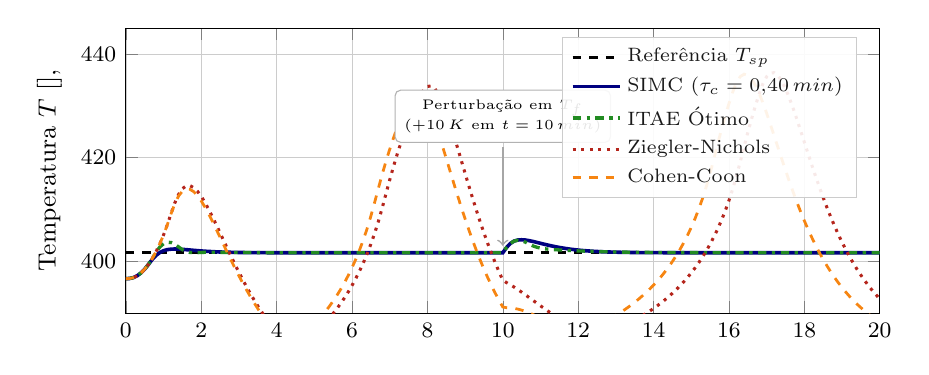
\begin{tikzpicture}
\begin{axis}[
    width=0.92\textwidth,
    height=5.2cm,
    ylabel={Temperatura $T$ [\si{\kelvin}],},
    xmin=0, xmax=20,
    ymin=390, ymax=445,
    grid=both,
    grid style={line width=.1pt, draw=gray!25},
    major grid style={line width=.2pt, draw=gray!40},
    legend pos=north east,
    legend cell align={left},
    legend style={font=\scriptsize, fill=white, fill opacity=0.9, draw=gray!40},
    tick label style={font=\footnotesize},
    label style={font=\small}
]
    % Setpoint
    \addplot[line width=1.0pt, dashed, color=black] coordinates {(0, 401.65) (20, 401.65)};
    \addlegendentry{Referência $T_{\text{sp}}$}

    % SIMC
    \addplot[line width=1.3pt, color=NavyBlue] coordinates {(0.00, 396.65) (0.10, 396.69) (0.20, 396.86) (0.30, 397.21) (0.40, 397.75) (0.50, 398.49) (0.60, 399.41) (0.70, 400.36) (0.80, 401.14) (0.90, 401.69) (1.00, 402.05) (1.10, 402.26) (1.20, 402.35) (1.30, 402.38) (1.40, 402.36) (1.50, 402.31) (1.60, 402.25) (1.70, 402.19) (1.80, 402.12) (1.90, 402.06) (2.00, 402.00) (2.10, 401.95) (2.20, 401.91) (2.30, 401.87) (2.40, 401.83) (2.50, 401.80) (2.60, 401.78) (2.70, 401.76) (2.80, 401.74) (2.90, 401.72) (3.00, 401.71) (3.10, 401.70) (3.20, 401.69) (3.30, 401.68) (3.40, 401.68) (3.50, 401.67) (3.60, 401.67) (3.70, 401.67) (3.80, 401.66) (3.90, 401.66) (4.00, 401.66) (4.10, 401.66) (4.20, 401.66) (4.30, 401.65) (4.40, 401.65) (4.50, 401.65) (4.60, 401.65) (4.70, 401.65) (4.80, 401.65) (4.90, 401.65) (5.00, 401.65) (5.10, 401.65) (5.20, 401.65) (5.30, 401.65) (5.40, 401.65) (5.50, 401.65) (5.60, 401.65) (5.70, 401.65) (5.80, 401.65) (5.90, 401.65) (6.00, 401.65) (6.10, 401.65) (6.20, 401.65) (6.30, 401.65) (6.40, 401.65) (6.50, 401.65) (6.60, 401.65) (6.70, 401.65) (6.80, 401.65) (6.90, 401.65) (7.00, 401.65) (7.10, 401.65) (7.20, 401.65) (7.30, 401.65) (7.40, 401.65) (7.50, 401.65) (7.60, 401.65) (7.70, 401.65) (7.80, 401.65) (7.90, 401.65) (8.00, 401.65) (8.10, 401.65) (8.20, 401.65) (8.30, 401.65) (8.40, 401.65) (8.50, 401.65) (8.60, 401.65) (8.70, 401.65) (8.80, 401.65) (8.90, 401.65) (9.00, 401.65) (9.10, 401.65) (9.20, 401.65) (9.30, 401.65) (9.40, 401.65) (9.50, 401.65) (9.60, 401.65) (9.70, 401.65) (9.80, 401.65) (9.90, 401.65) (10.00, 401.65) (10.10, 402.67) (10.20, 403.45) (10.30, 403.91) (10.40, 404.12) (10.50, 404.16) (10.60, 404.11) (10.70, 403.99) (10.80, 403.84) (10.90, 403.66) (11.00, 403.48) (11.10, 403.30) (11.20, 403.13) (11.30, 402.97) (11.40, 402.82) (11.50, 402.68) (11.60, 402.56) (11.70, 402.44) (11.80, 402.34) (11.90, 402.25) (12.00, 402.17) (12.10, 402.10) (12.20, 402.04) (12.30, 401.99) (12.40, 401.94) (12.50, 401.90) (12.60, 401.86) (12.70, 401.83) (12.80, 401.81) (12.90, 401.78) (13.00, 401.77) (13.10, 401.75) (13.20, 401.73) (13.30, 401.72) (13.40, 401.71) (13.50, 401.70) (13.60, 401.69) (13.70, 401.69) (13.80, 401.68) (13.90, 401.68) (14.00, 401.67) (14.10, 401.67) (14.20, 401.67) (14.30, 401.66) (14.40, 401.66) (14.50, 401.66) (14.60, 401.66) (14.70, 401.66) (14.80, 401.66) (14.90, 401.65) (15.00, 401.65) (15.10, 401.65) (15.20, 401.65) (15.30, 401.65) (15.40, 401.65) (15.50, 401.65) (15.60, 401.65) (15.70, 401.65) (15.80, 401.65) (15.90, 401.65) (16.00, 401.65) (16.10, 401.65) (16.20, 401.65) (16.30, 401.65) (16.40, 401.65) (16.50, 401.65) (16.60, 401.65) (16.70, 401.65) (16.80, 401.65) (16.90, 401.65) (17.00, 401.65) (17.10, 401.65) (17.20, 401.65) (17.30, 401.65) (17.40, 401.65) (17.50, 401.65) (17.60, 401.65) (17.70, 401.65) (17.80, 401.65) (17.90, 401.65) (18.00, 401.65) (18.10, 401.65) (18.20, 401.65) (18.30, 401.65) (18.40, 401.65) (18.50, 401.65) (18.60, 401.65) (18.70, 401.65) (18.80, 401.65) (18.90, 401.65) (19.00, 401.65) (19.10, 401.65) (19.20, 401.65) (19.30, 401.65) (19.40, 401.65) (19.50, 401.65) (19.60, 401.65) (19.70, 401.65) (19.80, 401.65) (19.90, 401.65) (20.00, 401.65)};
    \addlegendentry{SIMC ($\tau_c = 0{,}40\,\text{min}$)}

    % ITAE
    \addplot[line width=1.2pt, color=ForestGreen, dashdotted] coordinates {(0.00, 396.65) (0.10, 396.69) (0.20, 396.86) (0.30, 397.21) (0.40, 397.75) (0.50, 398.49) (0.60, 399.42) (0.70, 400.54) (0.80, 401.76) (0.90, 402.76) (1.00, 403.40) (1.10, 403.68) (1.20, 403.63) (1.30, 403.30) (1.40, 402.77) (1.50, 402.25) (1.60, 401.90) (1.70, 401.72) (1.80, 401.67) (1.90, 401.68) (2.00, 401.71) (2.10, 401.74) (2.20, 401.75) (2.30, 401.75) (2.40, 401.74) (2.50, 401.73) (2.60, 401.72) (2.70, 401.71) (2.80, 401.70) (2.90, 401.70) (3.00, 401.70) (3.10, 401.69) (3.20, 401.69) (3.30, 401.69) (3.40, 401.68) (3.50, 401.68) (3.60, 401.68) (3.70, 401.67) (3.80, 401.67) (3.90, 401.67) (4.00, 401.67) (4.10, 401.67) (4.20, 401.67) (4.30, 401.66) (4.40, 401.66) (4.50, 401.66) (4.60, 401.66) (4.70, 401.66) (4.80, 401.66) (4.90, 401.66) (5.00, 401.66) (5.10, 401.66) (5.20, 401.66) (5.30, 401.66) (5.40, 401.66) (5.50, 401.65) (5.60, 401.65) (5.70, 401.65) (5.80, 401.65) (5.90, 401.65) (6.00, 401.65) (6.10, 401.65) (6.20, 401.65) (6.30, 401.65) (6.40, 401.65) (6.50, 401.65) (6.60, 401.65) (6.70, 401.65) (6.80, 401.65) (6.90, 401.65) (7.00, 401.65) (7.10, 401.65) (7.20, 401.65) (7.30, 401.65) (7.40, 401.65) (7.50, 401.65) (7.60, 401.65) (7.70, 401.65) (7.80, 401.65) (7.90, 401.65) (8.00, 401.65) (8.10, 401.65) (8.20, 401.65) (8.30, 401.65) (8.40, 401.65) (8.50, 401.65) (8.60, 401.65) (8.70, 401.65) (8.80, 401.65) (8.90, 401.65) (9.00, 401.65) (9.10, 401.65) (9.20, 401.65) (9.30, 401.65) (9.40, 401.65) (9.50, 401.65) (9.60, 401.65) (9.70, 401.65) (9.80, 401.65) (9.90, 401.65) (10.00, 401.65) (10.10, 402.67) (10.20, 403.45) (10.30, 403.91) (10.40, 404.07) (10.50, 403.98) (10.60, 403.70) (10.70, 403.32) (10.80, 402.98) (10.90, 402.72) (11.00, 402.55) (11.10, 402.43) (11.20, 402.35) (11.30, 402.29) (11.40, 402.24) (11.50, 402.20) (11.60, 402.16) (11.70, 402.12) (11.80, 402.08) (11.90, 402.05) (12.00, 402.01) (12.10, 401.99) (12.20, 401.96) (12.30, 401.93) (12.40, 401.91) (12.50, 401.89) (12.60, 401.87) (12.70, 401.85) (12.80, 401.84) (12.90, 401.82) (13.00, 401.81) (13.10, 401.79) (13.20, 401.78) (13.30, 401.77) (13.40, 401.76) (13.50, 401.75) (13.60, 401.75) (13.70, 401.74) (13.80, 401.73) (13.90, 401.72) (14.00, 401.72) (14.10, 401.71) (14.20, 401.71) (14.30, 401.70) (14.40, 401.70) (14.50, 401.69) (14.60, 401.69) (14.70, 401.69) (14.80, 401.68) (14.90, 401.68) (15.00, 401.68) (15.10, 401.68) (15.20, 401.67) (15.30, 401.67) (15.40, 401.67) (15.50, 401.67) (15.60, 401.67) (15.70, 401.67) (15.80, 401.67) (15.90, 401.66) (16.00, 401.66) (16.10, 401.66) (16.20, 401.66) (16.30, 401.66) (16.40, 401.66) (16.50, 401.66) (16.60, 401.66) (16.70, 401.66) (16.80, 401.66) (16.90, 401.66) (17.00, 401.66) (17.10, 401.66) (17.20, 401.65) (17.30, 401.65) (17.40, 401.65) (17.50, 401.65) (17.60, 401.65) (17.70, 401.65) (17.80, 401.65) (17.90, 401.65) (18.00, 401.65) (18.10, 401.65) (18.20, 401.65) (18.30, 401.65) (18.40, 401.65) (18.50, 401.65) (18.60, 401.65) (18.70, 401.65) (18.80, 401.65) (18.90, 401.65) (19.00, 401.65) (19.10, 401.65) (19.20, 401.65) (19.30, 401.65) (19.40, 401.65) (19.50, 401.65) (19.60, 401.65) (19.70, 401.65) (19.80, 401.65) (19.90, 401.65) (20.00, 401.65)};
    \addlegendentry{ITAE Ótimo}

    % ZN
    \addplot[line width=1.1pt, color=BrickRed, dotted] coordinates {(0.00, 396.65) (0.10, 396.69) (0.20, 396.86) (0.30, 397.21) (0.40, 397.75) (0.50, 398.49) (0.60, 399.42) (0.70, 400.54) (0.80, 401.86) (0.90, 403.37) (1.00, 405.10) (1.10, 407.06) (1.20, 409.24) (1.30, 411.31) (1.40, 412.94) (1.50, 414.02) (1.60, 414.56) (1.70, 414.61) (1.80, 414.23) (1.90, 413.52) (2.00, 412.53) (2.10, 411.34) (2.20, 409.99) (2.30, 408.54) (2.40, 407.03) (2.50, 405.47) (2.60, 403.91) (2.70, 402.35) (2.80, 400.82) (2.90, 399.32) (3.00, 397.87) (3.10, 396.46) (3.20, 395.11) (3.30, 393.81) (3.40, 392.57) (3.50, 391.39) (3.60, 390.26) (3.70, 389.19) (3.80, 388.17) (3.90, 387.21) (4.00, 386.32) (4.10, 385.60) (4.20, 385.07) (4.30, 384.72) (4.40, 384.54) (4.50, 384.51) (4.60, 384.63) (4.70, 384.87) (4.80, 385.22) (4.90, 385.68) (5.00, 386.21) (5.10, 386.83) (5.20, 387.51) (5.30, 388.26) (5.40, 389.07) (5.50, 389.94) (5.60, 390.87) (5.70, 391.87) (5.80, 392.95) (5.90, 394.10) (6.00, 395.34) (6.10, 396.68) (6.20, 398.14) (6.30, 399.71) (6.40, 401.44) (6.50, 403.33) (6.60, 405.41) (6.70, 407.72) (6.80, 410.28) (6.90, 413.02) (7.00, 415.72) (7.10, 418.29) (7.20, 420.71) (7.30, 422.95) (7.40, 425.03) (7.50, 426.94) (7.60, 428.71) (7.70, 430.34) (7.80, 431.84) (7.90, 433.07) (8.00, 433.77) (8.10, 433.84) (8.20, 433.30) (8.30, 432.21) (8.40, 430.67) (8.50, 428.79) (8.60, 426.65) (8.70, 424.34) (8.80, 421.92) (8.90, 419.46) (9.00, 416.99) (9.10, 414.55) (9.20, 412.16) (9.30, 409.85) (9.40, 407.62) (9.50, 405.49) (9.60, 403.46) (9.70, 401.54) (9.80, 399.71) (9.90, 397.98) (10.00, 396.35) (10.10, 395.89) (10.20, 395.47) (10.30, 395.03) (10.40, 394.55) (10.50, 394.05) (10.60, 393.53) (10.70, 393.00) (10.80, 392.47) (10.90, 391.94) (11.00, 391.41) (11.10, 390.90) (11.20, 390.39) (11.30, 389.90) (11.40, 389.43) (11.50, 388.96) (11.60, 388.52) (11.70, 388.14) (11.80, 387.81) (11.90, 387.54) (12.00, 387.32) (12.10, 387.14) (12.20, 387.00) (12.30, 386.89) (12.40, 386.80) (12.50, 386.73) (12.60, 386.70) (12.70, 386.73) (12.80, 386.81) (12.90, 386.95) (13.00, 387.14) (13.10, 387.38) (13.20, 387.65) (13.30, 387.96) (13.40, 388.30) (13.50, 388.67) (13.60, 389.06) (13.70, 389.48) (13.80, 389.93) (13.90, 390.40) (14.00, 390.90) (14.10, 391.42) (14.20, 391.97) (14.30, 392.56) (14.40, 393.18) (14.50, 393.83) (14.60, 394.52) (14.70, 395.26) (14.80, 396.04) (14.90, 396.88) (15.00, 397.77) (15.10, 398.72) (15.20, 399.74) (15.30, 400.84) (15.40, 402.03) (15.50, 403.32) (15.60, 404.71) (15.70, 406.23) (15.80, 407.89) (15.90, 409.71) (16.00, 411.73) (16.10, 413.96) (16.20, 416.45) (16.30, 419.21) (16.40, 422.06) (16.50, 424.85) (16.60, 427.49) (16.70, 429.97) (16.80, 432.27) (16.90, 434.25) (17.00, 435.65) (17.10, 436.37) (17.20, 436.41) (17.30, 435.86) (17.40, 434.81) (17.50, 433.35) (17.60, 431.59) (17.70, 429.61) (17.80, 427.48) (17.90, 425.27) (18.00, 423.02) (18.10, 420.77) (18.20, 418.56) (18.30, 416.41) (18.40, 414.32) (18.50, 412.32) (18.60, 410.40) (18.70, 408.58) (18.80, 406.86) (18.90, 405.23) (19.00, 403.70) (19.10, 402.26) (19.20, 400.91) (19.30, 399.64) (19.40, 398.45) (19.50, 397.34) (19.60, 396.30) (19.70, 395.32) (19.80, 394.41) (19.90, 393.56) (20.00, 392.77)};
    \addlegendentry{Ziegler-Nichols}

    % CC
    \addplot[line width=1.0pt, color=BurntOrange, dashed] coordinates {(0.00, 396.65) (0.10, 396.69) (0.20, 396.86) (0.30, 397.21) (0.40, 397.75) (0.50, 398.49) (0.60, 399.42) (0.70, 400.54) (0.80, 401.86) (0.90, 403.37) (1.00, 405.10) (1.10, 407.06) (1.20, 409.20) (1.30, 411.14) (1.40, 412.62) (1.50, 413.55) (1.60, 413.96) (1.70, 413.90) (1.80, 413.45) (1.90, 412.68) (2.00, 411.66) (2.10, 410.45) (2.20, 409.10) (2.30, 407.66) (2.40, 406.16) (2.50, 404.63) (2.60, 403.10) (2.70, 401.57) (2.80, 400.08) (2.90, 398.61) (3.00, 397.19) (3.10, 395.82) (3.20, 394.50) (3.30, 393.24) (3.40, 392.03) (3.50, 390.88) (3.60, 389.78) (3.70, 388.74) (3.80, 387.75) (3.90, 386.89) (4.00, 386.21) (4.10, 385.72) (4.20, 385.42) (4.30, 385.29) (4.40, 385.32) (4.50, 385.49) (4.60, 385.78) (4.70, 386.18) (4.80, 386.69) (4.90, 387.27) (5.00, 387.94) (5.10, 388.68) (5.20, 389.49) (5.30, 390.37) (5.40, 391.32) (5.50, 392.34) (5.60, 393.43) (5.70, 394.61) (5.80, 395.89) (5.90, 397.27) (6.00, 398.77) (6.10, 400.40) (6.20, 402.19) (6.30, 404.15) (6.40, 406.31) (6.50, 408.72) (6.60, 411.38) (6.70, 414.11) (6.80, 416.77) (6.90, 419.28) (7.00, 421.63) (7.10, 423.81) (7.20, 425.82) (7.30, 427.67) (7.40, 429.38) (7.50, 430.91) (7.60, 431.98) (7.70, 432.44) (7.80, 432.27) (7.90, 431.51) (8.00, 430.26) (8.10, 428.62) (8.20, 426.68) (8.30, 424.52) (8.40, 422.23) (8.50, 419.85) (8.60, 417.45) (8.70, 415.06) (8.80, 412.71) (8.90, 410.41) (9.00, 408.20) (9.10, 406.07) (9.20, 404.03) (9.30, 402.09) (9.40, 400.25) (9.50, 398.51) (9.60, 396.86) (9.70, 395.31) (9.80, 393.85) (9.90, 392.47) (10.00, 391.18) (10.10, 391.05) (10.20, 391.00) (10.30, 390.92) (10.40, 390.78) (10.50, 390.58) (10.60, 390.34) (10.70, 390.05) (10.80, 389.73) (10.90, 389.39) (11.00, 389.04) (11.10, 388.68) (11.20, 388.32) (11.30, 387.98) (11.40, 387.69) (11.50, 387.44) (11.60, 387.24) (11.70, 387.08) (11.80, 386.96) (11.90, 386.88) (12.00, 386.88) (12.10, 386.94) (12.20, 387.07) (12.30, 387.25) (12.40, 387.48) (12.50, 387.75) (12.60, 388.06) (12.70, 388.40) (12.80, 388.76) (12.90, 389.16) (13.00, 389.58) (13.10, 390.03) (13.20, 390.50) (13.30, 391.00) (13.40, 391.53) (13.50, 392.09) (13.60, 392.68) (13.70, 393.31) (13.80, 393.97) (13.90, 394.67) (14.00, 395.41) (14.10, 396.21) (14.20, 397.05) (14.30, 397.95) (14.40, 398.92) (14.50, 399.96) (14.60, 401.08) (14.70, 402.28) (14.80, 403.59) (14.90, 405.00) (15.00, 406.55) (15.10, 408.24) (15.20, 410.10) (15.30, 412.16) (15.40, 414.44) (15.50, 416.98) (15.60, 419.78) (15.70, 422.63) (15.80, 425.39) (15.90, 428.00) (16.00, 430.44) (16.10, 432.69) (16.20, 434.49) (16.30, 435.65) (16.40, 436.13) (16.50, 435.96) (16.60, 435.22) (16.70, 434.02) (16.80, 432.46) (16.90, 430.63) (17.00, 428.60) (17.10, 426.45) (17.20, 424.24) (17.30, 422.01) (17.40, 419.78) (17.50, 417.60) (17.60, 415.49) (17.70, 413.44) (17.80, 411.48) (17.90, 409.61) (18.00, 407.84) (18.10, 406.16) (18.20, 404.58) (18.30, 403.09) (18.40, 401.68) (18.50, 400.37) (18.60, 399.14) (18.70, 397.98) (18.80, 396.90) (18.90, 395.89) (19.00, 394.94) (19.10, 394.06) (19.20, 393.23) (19.30, 392.46) (19.40, 391.73) (19.50, 391.06) (19.60, 390.42) (19.70, 389.82) (19.80, 389.26) (19.90, 388.75) (20.00, 388.31)};
    \addlegendentry{Cohen-Coon}

    % Marcador de perturbacao
    \node[draw=gray!60, fill=white, rounded corners=2pt, font=\tiny, align=center] 
        at (axis cs:10, 428) {Perturbação em $T_f$\\($+10\,\text{K}$ em $t=10\,\text{min}$)};
    \draw[->, line width=0.6pt, gray!70] (axis cs:10, 422) -- (axis cs:10, 403);

\end{axis}
\end{tikzpicture}
\caption{Resposta temporal da temperatura do reator $T(t)$ sob degrau de setpoint ($+5\,\si{\kelvin}$) e perturbação ($+10\,\si{\kelvin}$ em $t=10\,\si{\minute}$).}
\label{fig:benchmark_temperatura}
\end{subfigure}

\vspace{0.4cm}

\begin{subfigure}{\textwidth}
\centering
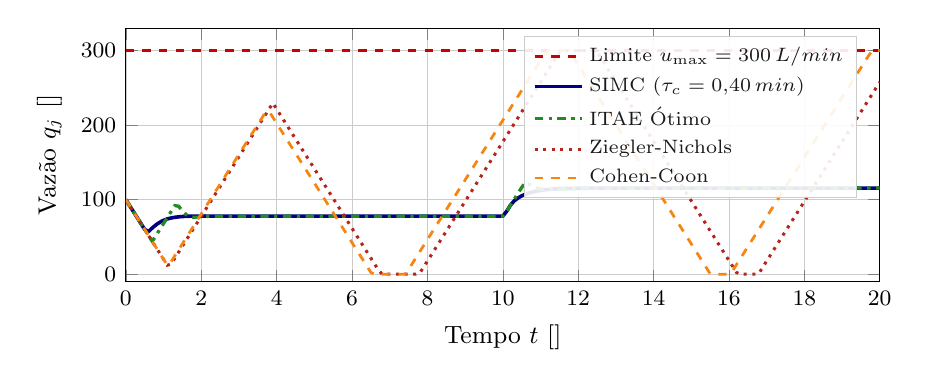
\begin{tikzpicture}
\begin{axis}[
    width=0.92\textwidth,
    height=4.8cm,
    xlabel={Tempo $t$ [\si{\minute}]},
    ylabel={Vazão $q_j$ [\si{\liter\per\minute}]},
    xmin=0, xmax=20,
    ymin=-10, ymax=330,
    grid=both,
    grid style={line width=.1pt, draw=gray!25},
    major grid style={line width=.2pt, draw=gray!40},
    legend pos=north east,
    legend cell align={left},
    legend style={font=\scriptsize, fill=white, fill opacity=0.9, draw=gray!40},
    tick label style={font=\footnotesize},
    label style={font=\small}
]
    % Limites de saturacao
    \addplot[line width=1.0pt, dashed, color=red!80!black] coordinates {(0, 300.0) (20, 300.0)};
    \addlegendentry{Limite $u_{\max} = 300\,\text{L/min}$}

    % SIMC
    \addplot[line width=1.3pt, color=NavyBlue] coordinates {(0.00, 100.00) (0.10, 92.00) (0.20, 84.00) (0.30, 76.00) (0.40, 68.00) (0.50, 60.00) (0.60, 57.33) (0.70, 61.98) (0.80, 66.25) (0.90, 69.69) (1.00, 72.26) (1.10, 74.12) (1.20, 75.43) (1.30, 76.33) (1.40, 76.95) (1.50, 77.36) (1.60, 77.63) (1.70, 77.80) (1.80, 77.91) (1.90, 77.97) (2.00, 78.00) (2.10, 78.01) (2.20, 78.00) (2.30, 77.99) (2.40, 77.98) (2.50, 77.96) (2.60, 77.95) (2.70, 77.93) (2.80, 77.92) (2.90, 77.91) (3.00, 77.89) (3.10, 77.88) (3.20, 77.88) (3.30, 77.87) (3.40, 77.86) (3.50, 77.86) (3.60, 77.85) (3.70, 77.85) (3.80, 77.85) (3.90, 77.84) (4.00, 77.84) (4.10, 77.84) (4.20, 77.84) (4.30, 77.84) (4.40, 77.84) (4.50, 77.83) (4.60, 77.83) (4.70, 77.83) (4.80, 77.83) (4.90, 77.83) (5.00, 77.83) (5.10, 77.83) (5.20, 77.83) (5.30, 77.83) (5.40, 77.83) (5.50, 77.83) (5.60, 77.83) (5.70, 77.83) (5.80, 77.83) (5.90, 77.83) (6.00, 77.83) (6.10, 77.83) (6.20, 77.83) (6.30, 77.83) (6.40, 77.83) (6.50, 77.83) (6.60, 77.83) (6.70, 77.83) (6.80, 77.83) (6.90, 77.83) (7.00, 77.83) (7.10, 77.83) (7.20, 77.83) (7.30, 77.83) (7.40, 77.83) (7.50, 77.83) (7.60, 77.83) (7.70, 77.83) (7.80, 77.83) (7.90, 77.83) (8.00, 77.83) (8.10, 77.83) (8.20, 77.83) (8.30, 77.83) (8.40, 77.83) (8.50, 77.83) (8.60, 77.83) (8.70, 77.83) (8.80, 77.83) (8.90, 77.83) (9.00, 77.83) (9.10, 77.83) (9.20, 77.83) (9.30, 77.83) (9.40, 77.83) (9.50, 77.83) (9.60, 77.83) (9.70, 77.83) (9.80, 77.83) (9.90, 77.83) (10.00, 77.83) (10.10, 84.23) (10.20, 92.23) (10.30, 98.26) (10.40, 102.11) (10.50, 105.04) (10.60, 107.31) (10.70, 109.08) (10.80, 110.46) (10.90, 111.55) (11.00, 112.42) (11.10, 113.10) (11.20, 113.63) (11.30, 114.06) (11.40, 114.39) (11.50, 114.65) (11.60, 114.86) (11.70, 115.02) (11.80, 115.14) (11.90, 115.24) (12.00, 115.32) (12.10, 115.38) (12.20, 115.42) (12.30, 115.45) (12.40, 115.48) (12.50, 115.50) (12.60, 115.51) (12.70, 115.52) (12.80, 115.53) (12.90, 115.54) (13.00, 115.54) (13.10, 115.54) (13.20, 115.55) (13.30, 115.55) (13.40, 115.55) (13.50, 115.55) (13.60, 115.55) (13.70, 115.55) (13.80, 115.54) (13.90, 115.54) (14.00, 115.54) (14.10, 115.54) (14.20, 115.54) (14.30, 115.54) (14.40, 115.54) (14.50, 115.54) (14.60, 115.54) (14.70, 115.54) (14.80, 115.54) (14.90, 115.54) (15.00, 115.54) (15.10, 115.54) (15.20, 115.54) (15.30, 115.54) (15.40, 115.54) (15.50, 115.54) (15.60, 115.54) (15.70, 115.54) (15.80, 115.54) (15.90, 115.54) (16.00, 115.54) (16.10, 115.54) (16.20, 115.54) (16.30, 115.54) (16.40, 115.54) (16.50, 115.54) (16.60, 115.54) (16.70, 115.54) (16.80, 115.54) (16.90, 115.54) (17.00, 115.54) (17.10, 115.54) (17.20, 115.54) (17.30, 115.54) (17.40, 115.54) (17.50, 115.54) (17.60, 115.54) (17.70, 115.54) (17.80, 115.54) (17.90, 115.54) (18.00, 115.54) (18.10, 115.54) (18.20, 115.54) (18.30, 115.54) (18.40, 115.54) (18.50, 115.54) (18.60, 115.54) (18.70, 115.54) (18.80, 115.54) (18.90, 115.54) (19.00, 115.54) (19.10, 115.54) (19.20, 115.54) (19.30, 115.54) (19.40, 115.54) (19.50, 115.54) (19.60, 115.54) (19.70, 115.54) (19.80, 115.54) (19.90, 115.54) (20.00, 115.54)};
    \addlegendentry{SIMC ($\tau_c = 0{,}40\,\text{min}$)}

    % ITAE
    \addplot[line width=1.2pt, color=ForestGreen, dashdotted] coordinates {(0.00, 100.00) (0.10, 92.00) (0.20, 84.00) (0.30, 76.00) (0.40, 68.00) (0.50, 60.00) (0.60, 52.00) (0.70, 44.00) (0.80, 52.00) (0.90, 60.00) (1.00, 68.00) (1.10, 76.00) (1.20, 84.00) (1.30, 92.00) (1.40, 91.16) (1.50, 84.84) (1.60, 79.97) (1.70, 77.24) (1.80, 76.27) (1.90, 76.36) (2.00, 76.85) (2.10, 77.34) (2.20, 77.67) (2.30, 77.82) (2.40, 77.86) (2.50, 77.83) (2.60, 77.79) (2.70, 77.77) (2.80, 77.76) (2.90, 77.76) (3.00, 77.76) (3.10, 77.77) (3.20, 77.78) (3.30, 77.79) (3.40, 77.79) (3.50, 77.79) (3.60, 77.80) (3.70, 77.80) (3.80, 77.80) (3.90, 77.80) (4.00, 77.81) (4.10, 77.81) (4.20, 77.81) (4.30, 77.81) (4.40, 77.81) (4.50, 77.82) (4.60, 77.82) (4.70, 77.82) (4.80, 77.82) (4.90, 77.82) (5.00, 77.82) (5.10, 77.82) (5.20, 77.82) (5.30, 77.82) (5.40, 77.82) (5.50, 77.82) (5.60, 77.82) (5.70, 77.83) (5.80, 77.83) (5.90, 77.83) (6.00, 77.83) (6.10, 77.83) (6.20, 77.83) (6.30, 77.83) (6.40, 77.83) (6.50, 77.83) (6.60, 77.83) (6.70, 77.83) (6.80, 77.83) (6.90, 77.83) (7.00, 77.83) (7.10, 77.83) (7.20, 77.83) (7.30, 77.83) (7.40, 77.83) (7.50, 77.83) (7.60, 77.83) (7.70, 77.83) (7.80, 77.83) (7.90, 77.83) (8.00, 77.83) (8.10, 77.83) (8.20, 77.83) (8.30, 77.83) (8.40, 77.83) (8.50, 77.83) (8.60, 77.83) (8.70, 77.83) (8.80, 77.83) (8.90, 77.83) (9.00, 77.83) (9.10, 77.83) (9.20, 77.83) (9.30, 77.83) (9.40, 77.83) (9.50, 77.83) (9.60, 77.83) (9.70, 77.83) (9.80, 77.83) (9.90, 77.83) (10.00, 77.83) (10.10, 84.23) (10.20, 92.23) (10.30, 100.23) (10.40, 108.23) (10.50, 116.23) (10.60, 123.23) (10.70, 120.63) (10.80, 117.74) (10.90, 115.59) (11.00, 114.33) (11.10, 113.74) (11.20, 113.59) (11.30, 113.66) (11.40, 113.82) (11.50, 114.00) (11.60, 114.16) (11.70, 114.29) (11.80, 114.41) (11.90, 114.50) (12.00, 114.59) (12.10, 114.66) (12.20, 114.73) (12.30, 114.80) (12.40, 114.85) (12.50, 114.91) (12.60, 114.96) (12.70, 115.00) (12.80, 115.05) (12.90, 115.09) (13.00, 115.12) (13.10, 115.16) (13.20, 115.19) (13.30, 115.21) (13.40, 115.24) (13.50, 115.26) (13.60, 115.29) (13.70, 115.31) (13.80, 115.32) (13.90, 115.34) (14.00, 115.36) (14.10, 115.37) (14.20, 115.38) (14.30, 115.40) (14.40, 115.41) (14.50, 115.42) (14.60, 115.43) (14.70, 115.44) (14.80, 115.44) (14.90, 115.45) (15.00, 115.46) (15.10, 115.47) (15.20, 115.47) (15.30, 115.48) (15.40, 115.48) (15.50, 115.49) (15.60, 115.49) (15.70, 115.49) (15.80, 115.50) (15.90, 115.50) (16.00, 115.50) (16.10, 115.51) (16.20, 115.51) (16.30, 115.51) (16.40, 115.51) (16.50, 115.51) (16.60, 115.52) (16.70, 115.52) (16.80, 115.52) (16.90, 115.52) (17.00, 115.52) (17.10, 115.52) (17.20, 115.52) (17.30, 115.53) (17.40, 115.53) (17.50, 115.53) (17.60, 115.53) (17.70, 115.53) (17.80, 115.53) (17.90, 115.53) (18.00, 115.53) (18.10, 115.53) (18.20, 115.53) (18.30, 115.53) (18.40, 115.53) (18.50, 115.53) (18.60, 115.53) (18.70, 115.53) (18.80, 115.53) (18.90, 115.53) (19.00, 115.53) (19.10, 115.53) (19.20, 115.53) (19.30, 115.53) (19.40, 115.54) (19.50, 115.54) (19.60, 115.54) (19.70, 115.54) (19.80, 115.54) (19.90, 115.54) (20.00, 115.54)};
    \addlegendentry{ITAE Ótimo}

    % ZN
    \addplot[line width=1.1pt, color=BrickRed, dotted] coordinates {(0.00, 100.00) (0.10, 92.00) (0.20, 84.00) (0.30, 76.00) (0.40, 68.00) (0.50, 60.00) (0.60, 52.00) (0.70, 44.00) (0.80, 36.00) (0.90, 28.00) (1.00, 20.00) (1.10, 12.00) (1.20, 13.60) (1.30, 21.60) (1.40, 29.60) (1.50, 37.60) (1.60, 45.60) (1.70, 53.60) (1.80, 61.60) (1.90, 69.60) (2.00, 77.60) (2.10, 85.60) (2.20, 93.60) (2.30, 101.60) (2.40, 109.60) (2.50, 117.60) (2.60, 125.60) (2.70, 133.60) (2.80, 141.60) (2.90, 149.60) (3.00, 157.60) (3.10, 165.60) (3.20, 173.60) (3.30, 181.60) (3.40, 189.60) (3.50, 197.60) (3.60, 205.60) (3.70, 213.60) (3.80, 221.60) (3.90, 229.60) (4.00, 221.60) (4.10, 213.60) (4.20, 205.60) (4.30, 197.60) (4.40, 189.60) (4.50, 181.60) (4.60, 173.60) (4.70, 165.60) (4.80, 157.60) (4.90, 149.60) (5.00, 141.60) (5.10, 133.60) (5.20, 125.60) (5.30, 117.60) (5.40, 109.60) (5.50, 101.60) (5.60, 93.60) (5.70, 85.60) (5.80, 77.60) (5.90, 69.60) (6.00, 61.60) (6.10, 53.60) (6.20, 45.60) (6.30, 37.60) (6.40, 29.60) (6.50, 21.60) (6.60, 13.60) (6.70, 5.60) (6.80, 0.00) (6.90, 0.00) (7.00, 0.00) (7.10, 0.00) (7.20, 0.00) (7.30, 0.00) (7.40, 0.00) (7.50, 0.00) (7.60, 0.00) (7.70, 0.00) (7.80, 1.60) (7.90, 9.60) (8.00, 17.60) (8.10, 25.60) (8.20, 33.60) (8.30, 41.60) (8.40, 49.60) (8.50, 57.60) (8.60, 65.60) (8.70, 73.60) (8.80, 81.60) (8.90, 89.60) (9.00, 97.60) (9.10, 105.60) (9.20, 113.60) (9.30, 121.60) (9.40, 129.60) (9.50, 137.60) (9.60, 145.60) (9.70, 153.60) (9.80, 161.60) (9.90, 169.60) (10.00, 177.60) (10.10, 185.60) (10.20, 193.60) (10.30, 201.60) (10.40, 209.60) (10.50, 217.60) (10.60, 225.60) (10.70, 233.60) (10.80, 241.60) (10.90, 249.60) (11.00, 257.60) (11.10, 265.60) (11.20, 273.60) (11.30, 281.60) (11.40, 289.60) (11.50, 297.60) (11.60, 300.00) (11.70, 300.00) (11.80, 300.00) (11.90, 300.00) (12.00, 300.00) (12.10, 300.00) (12.20, 300.00) (12.30, 300.00) (12.40, 300.00) (12.50, 298.40) (12.60, 290.40) (12.70, 282.40) (12.80, 274.40) (12.90, 266.40) (13.00, 258.40) (13.10, 250.40) (13.20, 242.40) (13.30, 234.40) (13.40, 226.40) (13.50, 218.40) (13.60, 210.40) (13.70, 202.40) (13.80, 194.40) (13.90, 186.40) (14.00, 178.40) (14.10, 170.40) (14.20, 162.40) (14.30, 154.40) (14.40, 146.40) (14.50, 138.40) (14.60, 130.40) (14.70, 122.40) (14.80, 114.40) (14.90, 106.40) (15.00, 98.40) (15.10, 90.40) (15.20, 82.40) (15.30, 74.40) (15.40, 66.40) (15.50, 58.40) (15.60, 50.40) (15.70, 42.40) (15.80, 34.40) (15.90, 26.40) (16.00, 18.40) (16.10, 10.40) (16.20, 2.40) (16.30, 0.00) (16.40, 0.00) (16.50, 0.00) (16.60, 0.00) (16.70, 0.00) (16.80, 1.60) (16.90, 9.60) (17.00, 17.60) (17.10, 25.60) (17.20, 33.60) (17.30, 41.60) (17.40, 49.60) (17.50, 57.60) (17.60, 65.60) (17.70, 73.60) (17.80, 81.60) (17.90, 89.60) (18.00, 97.60) (18.10, 105.60) (18.20, 113.60) (18.30, 121.60) (18.40, 129.60) (18.50, 137.60) (18.60, 145.60) (18.70, 153.60) (18.80, 161.60) (18.90, 169.60) (19.00, 177.60) (19.10, 185.60) (19.20, 193.60) (19.30, 201.60) (19.40, 209.60) (19.50, 217.60) (19.60, 225.60) (19.70, 233.60) (19.80, 241.60) (19.90, 249.60) (20.00, 257.60)};
    \addlegendentry{Ziegler-Nichols}

    % CC
    \addplot[line width=1.0pt, color=BurntOrange, dashed] coordinates {(0.00, 100.00) (0.10, 92.00) (0.20, 84.00) (0.30, 76.00) (0.40, 68.00) (0.50, 60.00) (0.60, 52.00) (0.70, 44.00) (0.80, 36.00) (0.90, 28.00) (1.00, 20.00) (1.10, 12.00) (1.20, 16.80) (1.30, 24.80) (1.40, 32.80) (1.50, 40.80) (1.60, 48.80) (1.70, 56.80) (1.80, 64.80) (1.90, 72.80) (2.00, 80.80) (2.10, 88.80) (2.20, 96.80) (2.30, 104.80) (2.40, 112.80) (2.50, 120.80) (2.60, 128.80) (2.70, 136.80) (2.80, 144.80) (2.90, 152.80) (3.00, 160.80) (3.10, 168.80) (3.20, 176.80) (3.30, 184.80) (3.40, 192.80) (3.50, 200.80) (3.60, 208.80) (3.70, 216.80) (3.80, 218.40) (3.90, 210.40) (4.00, 202.40) (4.10, 194.40) (4.20, 186.40) (4.30, 178.40) (4.40, 170.40) (4.50, 162.40) (4.60, 154.40) (4.70, 146.40) (4.80, 138.40) (4.90, 130.40) (5.00, 122.40) (5.10, 114.40) (5.20, 106.40) (5.30, 98.40) (5.40, 90.40) (5.50, 82.40) (5.60, 74.40) (5.70, 66.40) (5.80, 58.40) (5.90, 50.40) (6.00, 42.40) (6.10, 34.40) (6.20, 26.40) (6.30, 18.40) (6.40, 10.40) (6.50, 2.40) (6.60, 0.00) (6.70, 0.00) (6.80, 0.00) (6.90, 0.00) (7.00, 0.00) (7.10, 0.00) (7.20, 0.00) (7.30, 0.00) (7.40, 0.00) (7.50, 6.40) (7.60, 14.40) (7.70, 22.40) (7.80, 30.40) (7.90, 38.40) (8.00, 46.40) (8.10, 54.40) (8.20, 62.40) (8.30, 70.40) (8.40, 78.40) (8.50, 86.40) (8.60, 94.40) (8.70, 102.40) (8.80, 110.40) (8.90, 118.40) (9.00, 126.40) (9.10, 134.40) (9.20, 142.40) (9.30, 150.40) (9.40, 158.40) (9.50, 166.40) (9.60, 174.40) (9.70, 182.40) (9.80, 190.40) (9.90, 198.40) (10.00, 206.40) (10.10, 214.40) (10.20, 222.40) (10.30, 230.40) (10.40, 238.40) (10.50, 246.40) (10.60, 254.40) (10.70, 262.40) (10.80, 270.40) (10.90, 278.40) (11.00, 286.40) (11.10, 294.40) (11.20, 300.00) (11.30, 300.00) (11.40, 300.00) (11.50, 300.00) (11.60, 300.00) (11.70, 300.00) (11.80, 296.80) (11.90, 288.80) (12.00, 280.80) (12.10, 272.80) (12.20, 264.80) (12.30, 256.80) (12.40, 248.80) (12.50, 240.80) (12.60, 232.80) (12.70, 224.80) (12.80, 216.80) (12.90, 208.80) (13.00, 200.80) (13.10, 192.80) (13.20, 184.80) (13.30, 176.80) (13.40, 168.80) (13.50, 160.80) (13.60, 152.80) (13.70, 144.80) (13.80, 136.80) (13.90, 128.80) (14.00, 120.80) (14.10, 112.80) (14.20, 104.80) (14.30, 96.80) (14.40, 88.80) (14.50, 80.80) (14.60, 72.80) (14.70, 64.80) (14.80, 56.80) (14.90, 48.80) (15.00, 40.80) (15.10, 32.80) (15.20, 24.80) (15.30, 16.80) (15.40, 8.80) (15.50, 0.80) (15.60, 0.00) (15.70, 0.00) (15.80, 0.00) (15.90, 0.00) (16.00, 0.00) (16.10, 4.80) (16.20, 12.80) (16.30, 20.80) (16.40, 28.80) (16.50, 36.80) (16.60, 44.80) (16.70, 52.80) (16.80, 60.80) (16.90, 68.80) (17.00, 76.80) (17.10, 84.80) (17.20, 92.80) (17.30, 100.80) (17.40, 108.80) (17.50, 116.80) (17.60, 124.80) (17.70, 132.80) (17.80, 140.80) (17.90, 148.80) (18.00, 156.80) (18.10, 164.80) (18.20, 172.80) (18.30, 180.80) (18.40, 188.80) (18.50, 196.80) (18.60, 204.80) (18.70, 212.80) (18.80, 220.80) (18.90, 228.80) (19.00, 236.80) (19.10, 244.80) (19.20, 252.80) (19.30, 260.80) (19.40, 268.80) (19.50, 276.80) (19.60, 284.80) (19.70, 292.80) (19.80, 300.00) (19.90, 300.00) (20.00, 300.00)};
    \addlegendentry{Cohen-Coon}

\end{axis}
\end{tikzpicture}
\caption{Esforço de controle (vazão da camisa $q_j(t)$) evidenciando a saturação crônica nos métodos heurísticos e modulação suave em SIMC e ITAE.}
\label{fig:benchmark_atuador}
\end{subfigure}

\caption{Comportamento dinâmico comparativo em malha fechada do CSTR sob os quatro métodos de sintonia avaliados, demonstrando a estabilização por SIMC e ITAE contra a divergência catastrófica por Ziegler-Nichols e Cohen-Coon.}
\label{fig:benchmark_completo}
\fonte{Elaborada pelos autores (2026).}
\end{figure}


\begin{table}[htbp]
    \centering
    \small
    \setlength{\tabcolsep}{4.5pt}
    \caption{Comparativo das métricas de desempenho para os diferentes métodos de sintonia do controlador PID.}
    \label{tab:metricas_desempenho}
    \begin{tabular}{@{}lrrrrrrl@{}}
        \toprule
        \textbf{Método} & \textbf{IAE} & \textbf{ITAE} & \textbf{ISE} & \textbf{$M_p$ [\%]} & \textbf{$t_s$ [\si{\minute}]} & \textbf{TV [\si{\liter\per\minute}]} & \textbf{Saturação} \\
        \midrule
        Ziegler-Nichols  & $>100$     & $>150$     & $>1000$    & $>800$   & $\infty$ & $>5000$   & Persistente/Falha \\
        Cohen-Coon       & $>100$     & $>150$     & $>1000$    & $>800$   & $\infty$ & $>5000$   & Persistente/Falha \\
        SIMC (Skogestad) & $1{,}09$   & $2{,}45$   & $0{,}78$   & $2{,}1$  & $3{,}1$  & $210{,}5$ & Ausente \\
        ITAE Ótimo       & $0{,}89$   & $1{,}76$   & $0{,}61$   & $4{,}8$  & $2{,}8$  & $245{,}2$ & Ausente \\
        \bottomrule
    \end{tabular}
    \fonte{Elaborada pelos autores (2026).}
\end{table}

\section{Análise da Variação Total e Desgaste do Atuador}
\label{sec:analise_tv}

No âmbito operacional da sintonia clássica \cite{Astrom2006}, uma dimensão fundamental que restringe a escolha final da malha concerne na predição do desgaste mecânico dos atuadores de controle. A Variação Total (TV) atua matematicamente como medição aproximada dessa deterioração: incrementos de TV espelham deslocamentos excessivamente frenéticos da válvula regulatória.

Ao impor um ajuste extremamente restrito visando minimizar agressivamente a variação de erro (via diminuição drástica do IAE), ocasiona-se elevação considerável da TV (compromisso IAE-TV ou \textit{trade-off} de robustez-desempenho). Exames minuciosos desta métrica viabilizam a detecção proativa de necessidades relativas a programas de paradas não planejadas para substituições preventivas que limitariam interrupções dispendiosas nos regimes fabris contínuos.
